\section{Розробка підходу до вирішення завдання}

\subsection{Огляд аналогів}
magic table
%TODO: Огляд аналогів

\subsection{Схема розв’язання}
% TODO: додати в другий розділ щось, де визначається пропускна здатність
Задача моєї дипломної роботи полягає в визначенні пропускної здатності маркетингового каналу. Для виконання задачі необхідно отримати перспективну інформацію щодо функціонування каналу та проаналізувати її. Схема розв’язання задачі зображена на рисунку \ref{fig:solution_schema}.

Пропонується прогнозувати діяльність маркетингового каналу за допомогою імітаційного моделювання. В перших двох діях на діаграмі активностей формується склад учасників гри та структура каналу, що моделюється; третьою дією будується імітаційна модель. Після того як модель побудована, можна проводити імітаційний експеримент (дія №4), який буде генерувати вихідні дані, що будуть проаналізовані.

            \begin{stdfigure}
                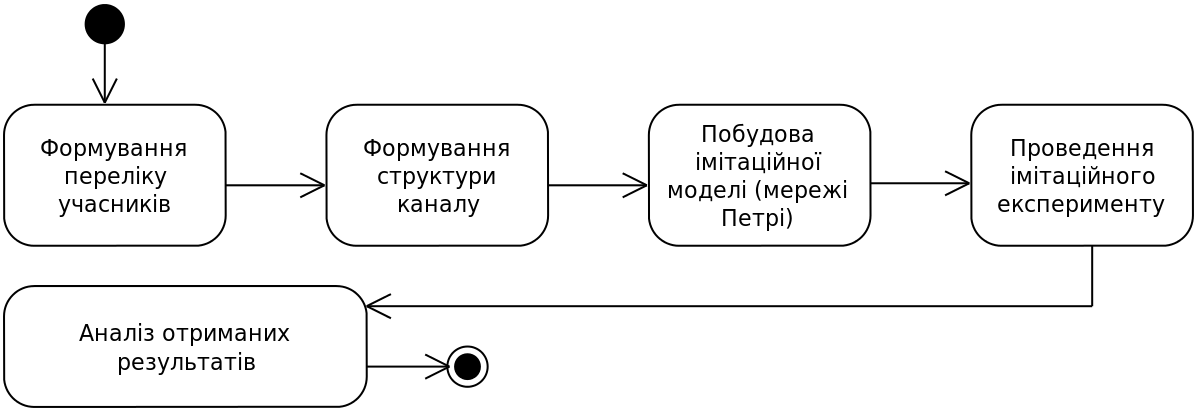
\includegraphics[width=2in]{images/uml_act_solution_schema.png}
                \caption{Схема розв’язання задачі в вигляді діаграми активностей}
                \label{fig:solution_schema}
            \end{stdfigure}   
\subsection{Імітаційне моделювання}
\subsubsection{Огляд}
Моделювання --- це процесс побудови моделі для заміни досліджуємого об’єкту з метою дослідження його властивостей, прогнозування поведінки на основі властивостей моделі та характеристик її поведінки\cite{model}.

В залежності від характеру досліджуємих процесів всі види моделювання можуть бути розділені на:
\begin{enumerate}
\item детерміновані та стохастичні;
\item статичні та динамічні;
\item дискретні, безперервні та дискретно-безперервні;
\end{enumerate}
 
Детерміноване модeлювання відображає детерміновані процеси, тобто процеси, в яких передбачається відсутність будь-яких випадкових впливів; стохастичне моделювання відображає імовірнісні процеси та події. Статичне моделювання служить для описання поведінки моделі в будь-який момент часу, а динамічне відображає поведінку об’єкту в часі. Дискретне моделювання відображає дискретні процеси, а безперервне -- безперервні процеси\cite{model}.

Виділяють наступні основні методи моделювання\cite{model}:
\begin{longEnumerate}
   \item Математичне моделювання --- процес встановлення відповідності даному реальному об’єкту деякого математичного об’єкту, що називається математичною моделлю, та дослідження цієї моделі, що дозволяює отримувати характеристики об’єкта. 
   \item Аналітичне моделювання. В аналітичному моделюванні процеси записуються в вигляді функціональніх співвідношень та логичніх умов.
   \item Імітаційне моделювання. В цьому виді моделювання алгоритм, що реалізує модель, відтворює процес функціонування системи у часі.
   \item Комбіноване моделювання -- при будуванні комбінованих моделей для деяких складових процесу використовують аналітичні моделі, а для інших --- імітаційні.
\end{longEnumerate}

Імітаційне моделювання дозволяє досліджувати більш складні системи, ніж аналітичне моделювання. Імітаційна модель може відображати дискретність, нелінійність, недетермінованість та інші якості системи, які неможливо врахувати в аналітичних моделях. 

\subsubsection{Мережі Петрі}
Мережа Петрі --- це математичний апарат для моделювання динамічних дискретних систем. Мережею Петрі називають двудольний орієнтований граф \mbox {$ N = \langle P, T, * \rangle $}, де \mbox{$ P = \{p_i\}, T = \{t_i\} $} --- кінцеві непусті множини вершин, що називаються відповідно позиціями та переходами; $*$ --- відношення між вершинам, що відповідають дугам графа. Позиції зображаються кружками, переходи --- рисками. Дуги з’єднують кружки з рисками чи навпаки, але не вершини однакового типу.

Маркуванням мережі Петрі називається функція $F$, яка кожній позиції ставить в відповідність ціле позитивне не негативне число. Маркування характеризується вектором \mbox{$ F = \langle F(p_1), \dots, F(p_n) \rangle $}, де $n$ --- число позицій в мережі.
% TODO: переписати Мережі Петрі за Совєтовим! Сорець не забути
Різні маркування мережі Петрі характеризують стани відповідної динамічної системи, де динаміка моделюється рухом меток по позиціях.

Якщо кожна з вхідних позицій перехода $t$ складається з якомога однією мітки, то перехід $t$ може спрацювати. При спрацюванні переходу з кожної його вхідної позиції видаляється одна мітка, а в кожну вихідну додається.

            \begin{stdfigure}
                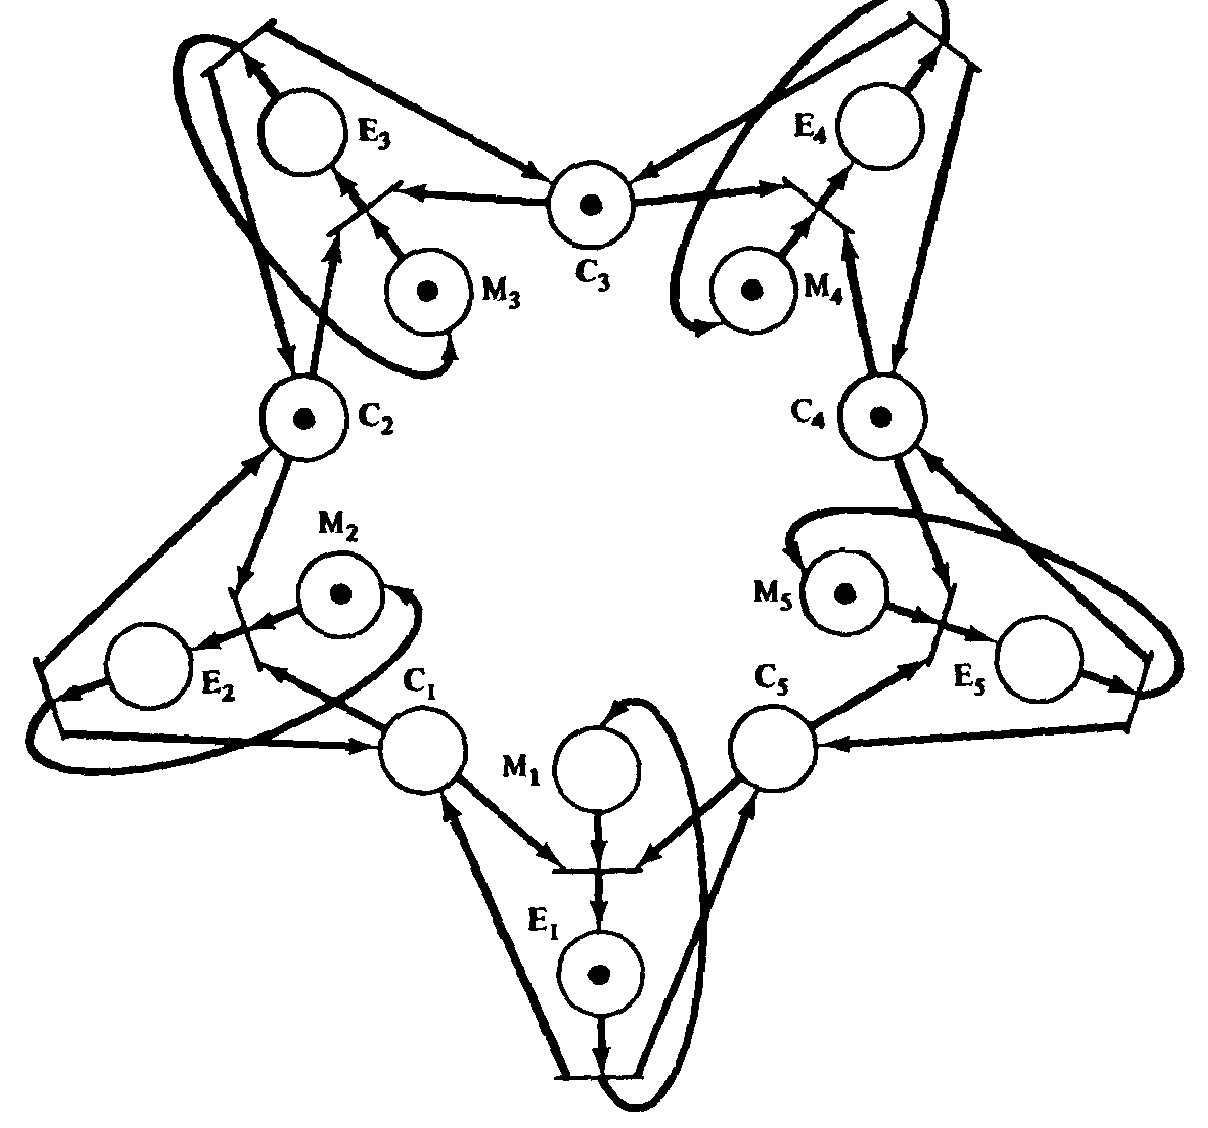
\includegraphics[width=4in]{images/petri_net_example.png}
                \caption{Приклад мережі Петрі}
                \label{fig:petri_net_example}
            \end{stdfigure}   

% безпечні мережі петри
%При применении сетей Петри для целей управления позициям сопос­
%тавляются операции (действия), а переходам — условия, при выполнении
%которых возбужденные переходы срабатывают, активизируя соответству­
%ющие операции [31]. При этом попадание меток в позицию ассоциируется
%с началом операции, а удаление метки — с ее окончанием. При исполь­
%зовании такого предположения считают, что любая операция не может
%быть повторно начата до ее завершения. Для описания таких процессов
%могут применяться только б е з о п а с н ы е сети Петри, т. е. такие сети, в
%которых при любой маркировке в каждой позиции не может быть более
%одной метки.
\subsection{Теорія ділових ігор}
\subsubsection{Огляд}
Гра --- це вид людської діяльності, що здатен відтворювати інші види людської діяльності. Імітаційна гра або ділова гра --- гра, що є імітаційною моделлю, яка призначена для вивчення процесів функціонування організаційно-економічних систем. Імітаційними іграми називають такі ігри, в яких важливою частиною відтворення експериментальної ситуації є імітаційна модель середи, в якій виконавці ролей здійснюють свою діяльність\cite{aristov}. Ділова імітаційна гра є ефективним засобом перевірки властивостей економічних систем \cite{burkov}.

Для використання ділових ігор в дослідницьких цілях, використовують ігри з участю автоматів \cite{burkov}. В таких іграх частина учасників гри замінюється автоматами (під автоматом мається на увазі програма, що моделює діяльність людини) з формалізованими процедурами прийняття рішень. Використання автоматів пов’язано з тим, що автомат здатен приймати рішення швидше за людину, що дозволяє зкоротити тривалість однієї партії.

            \begin{stdfigure}
                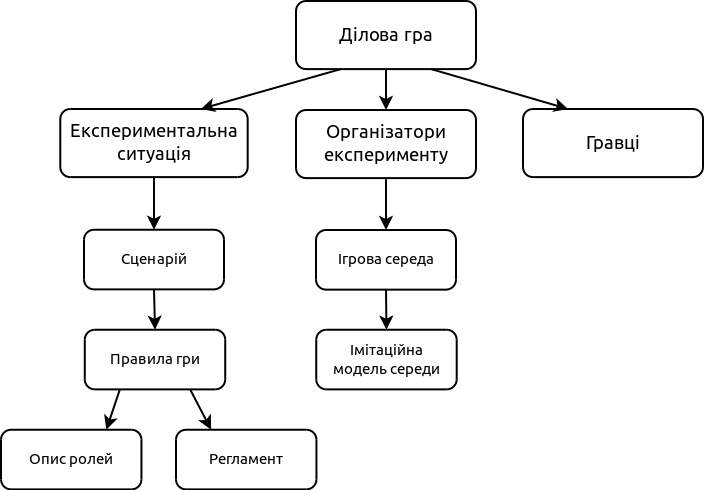
\includegraphics[width=6in]{images/game.png}
                \caption{Компоненти ділової гри\cite{aristov}}
                \label{fig:game}
            \end{stdfigure}   

\subsubsection{Склад ділової гри <<Маркетинговий канал>>}
Ділова гра, в загальному випадку, складається з трьох компонентів: опису експериментальної ситуації, організаційної частини та гравців. Експериментальна ситуація описується необов’язковим сценарієм гри, регламентом гри та описом ролей гравців. Організаційна частина --- це середа, в якій відбувається гра або імітаційна модель цієї середи. Третья частина, гравці --- це перелік всіх учасників ділової гри, між якими будуть розподілені ігрові ролі.

Ділова гра <<Маркетинговий канал>> розподіляє гравців на чотири ролі, що відповідають видам учасників маркетингових канадів, це: <<виробники (producers)>>, <<дистриб’ютори (distributors)>>, <<рітейлери (retailers)>>, <<клієнти (clients)>>. Кожен гравець може мати тільки одну роль.

Визначимо правила гри. Ділова гра є пошаговою грою та проходить циклічно. Кожна ітерація ігрового циклу складається з чотирьох шагів. На кожному з шагів всі представники відповідної ролі роблять хід, після чого право ходу переходить до наступної ролі. Послідовніть шагів в ітерації:
\begin{enumerate} % TODO: clarify порядок
\item <<виробники>>;
\item <<дистриб’ютори>>;
\item <<рітейлери>>;
\item <<клієнти>>.
\end{enumerate}

В процесі гри гравці обмінюються замовленнями на товар або виробляють його. Відповідно до принципів побудування структури маркетингових каналів, існують наступні обмеження на взаємодію гравців: <<клієнти>> можуть робити замовлення тільки у <<рітейлерів>>, <<рітейлери>> у <<дистриб’юторів>>, <<дистриб’ютор>> у <<виробників>>, а <<виробники>> безпосередньо виробляють товар.

Гра відбувається у визначенному проміжку часу, після спливу якого вона зупиняється. Після кожного ходу повинен проводитися аналіз ігрової ситуації, за результатами якого гра також може бути зупинена. Гра повинна бути зупинена, якщо: 
\begin{enumerate}
\item один із гравців не зміг обробити всі вхідні замовлення.
\end{enumerate}
 
Як визначено у розділі 1.2.3, метою моделювання є визначення пропускної здатності каналу, а об’єктом моделювання є маркетинговий канал. Виходячи з цього, визначаємо ігровою середою модель структури маркетингового каналу. Перелік гравців та структура маркетингового каналу визначається організатором гри.

\subsection{Побудова моделі}
\subsubsection{Алгоритм побудови моделі}
% Простым и доступным текстом вроде:
%В примере рассматривается описание двух взаимодействующих процессов на основе механизма семафоров. Пусть в общей памяти выделен участок длиною единиц, который используется для хранения запросов на выполнение задач. Процессы записи запросов в очередь и выбора их из очереди могут происходить независимо (асинхронно). Описатель очереди содержит четыре элемента: и - число заполненных и свободных ячеек очереди; и - адреса начального и конечного элементов очереди. Алгоритмы записи в очередь и выборки запросов из очереди приведены на рис. 5.9. Запись вида представляет операцию размещения в ячейку очереди с номером , а запись вида - считывание содержимого ячейки и использование его в качестве информации о запросе.
 
% Матаном. Сеть -- это четверка, вектор такой, векторй сякой. Маркировка сети, графы достижимости.


%TODO: Алгоритм побудови моделі

% то є реальна модель, що будет реалізована у вигляді мережі Петрі
% відповідно до постановки задачі, моделюємо маркетинговий канал.
% згадаємо про його структуру
%  маркер -- єто флажок (yep), что ход у єтого игрока или он отображает реальное количество произведенного товара?
\subsubsection{Алгоритм проведення експерименту}
% TODO: Алгоритм проведення експ.?
% Було б гарно, якщо б більша частина алгоритму була мережею Петрі
\subsection{Виводи до розділу}
Обосновать выбор імітации, сети петрі, декловой игрі.


%TODO: Виводи до розділу
 
